\documentclass[border=3pt]{standalone}
\usepackage[T1]{fontenc}
\usepackage{lmodern,amsmath,amssymb,tikz}
\usetikzlibrary{arrows.meta,calc,positioning,backgrounds,shapes.geometric}
\definecolor{ink}{HTML}{20344A}
\definecolor{muted}{HTML}{68798B}
\definecolor{linecol}{HTML}{B4C0CB}
\definecolor{teal}{HTML}{177E89}
\definecolor{pale}{HTML}{EAF5F5}
\definecolor{blue}{HTML}{4F78AE}
\definecolor{bluep}{HTML}{EDF2FA}
\definecolor{gold}{HTML}{B78227}
\definecolor{goldp}{HTML}{FCF5E7}
\definecolor{purple}{HTML}{846BA1}
\definecolor{purplep}{HTML}{F2EDF7}
\tikzset{
 arr/.style={-{Stealth[length=1.8mm,width=1.25mm]},draw=ink!75,line width=.65pt,rounded corners=1pt},
 guide/.style={draw=linecol,line width=.55pt},
 heading/.style={font=\sffamily\bfseries\small,text=ink,anchor=west},
 lab/.style={font=\sffamily\footnotesize,text=ink,align=center,inner sep=1pt},
 sub/.style={font=\sffamily\scriptsize,text=muted,align=center,inner sep=1pt},
 dot/.style={circle,draw=blue!80,fill=white,minimum size=4.8mm,inner sep=0pt,font=\sffamily\scriptsize,text=blue},
 card/.style={rounded corners=2pt,line width=.65pt,draw=blue!70,fill=bluep,minimum width=2.35cm,minimum height=.54cm,font=\sffamily\footnotesize,text=ink,inner sep=2pt},
}
\newcommand{\tensor}[5]{%
\begin{scope}[shift={(#1,#2)}]
\filldraw[draw=#5!85,fill=#5!13,line width=.6pt] (-#3/2,-#4/2) rectangle (#3/2,#4/2);
\filldraw[draw=#5!85,fill=#5!27,line width=.6pt] (#3/2,-#4/2)--++(.14,.12)--++(0,#4)--++(-.14,-.12)--cycle;
\filldraw[draw=#5!85,fill=#5!8,line width=.6pt] (-#3/2,#4/2)--++(.14,.12)--++(#3,0)--++(-.14,-.12)--cycle;
\draw[#5!35,line width=.4pt] (-#3/6,-#4/2)--(-#3/6,#4/2) (#3/6,-#4/2)--(#3/6,#4/2);
\end{scope}}
\newcommand{\frameicon}[3]{%
\begin{scope}[shift={(#1,#2)},scale=#3]
\filldraw[rounded corners=2pt,draw=ink!60,fill=ink!6,line width=.65pt] (-.92,-.65) rectangle (.92,.65);
\fill[teal!10] (0,0) ellipse (.78 and .52);
\draw[draw=ink!50,line width=3pt,line cap=round] (-.86,-.43)--(-.18,.04) (.88,.43)--(.29,.04);
\draw[draw=ink!70,line width=.8pt] (-.18,.04)--(-.02,.14)--(.08,.07) (-.18,.04)--(-.05,-.08)--(.06,-.03);
\draw[draw=ink!70,line width=.8pt] (.29,.04)--(.11,.18)--(.03,.13) (.29,.04)--(.14,-.10)--(.06,-.06);
\end{scope}}
\newcommand{\head}[2]{%
\begin{scope}[shift={(#1,#2)}]
\filldraw[fill=goldp,draw=gold!80,rounded corners=1pt,line width=.6pt] (-.74,-.23) rectangle (.08,.23);
\draw[gold,line width=.65pt] (-.53,-.10) rectangle (-.13,.11);
\filldraw[fill=purplep,draw=purple!80,rounded corners=1pt,line width=.6pt] (.14,-.23) rectangle (.88,.23);
\foreach \x/\h in {.30/.12,.46/.23,.62/.32}{\fill[purple!70] (\x,-.15) rectangle ++(.08,\h);}
\end{scope}}
\begin{document}
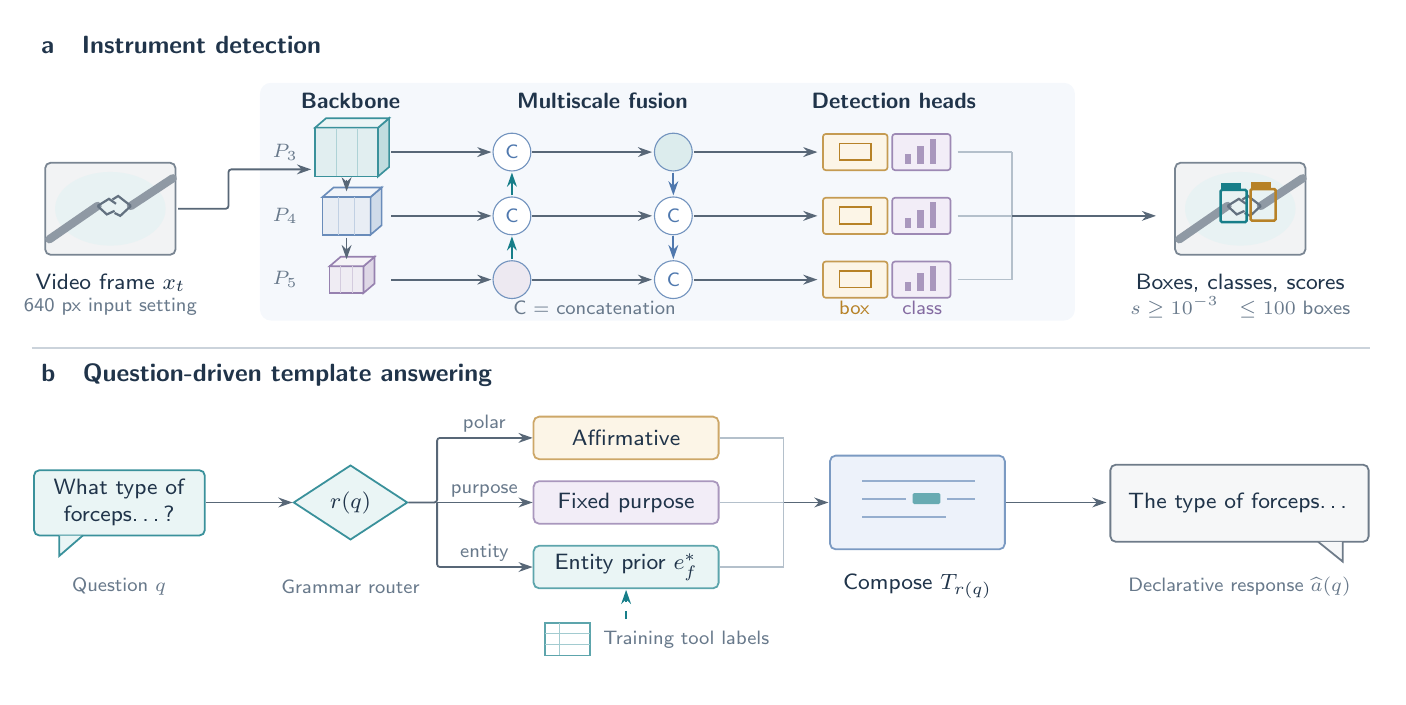
\begin{tikzpicture}[x=1cm,y=1cm]
\path[use as bounding box] (-.05,-.05) rectangle (17.1,8.2);
\node[heading] at (0,7.98) {a\quad Instrument detection};

\fill[bluep!55,rounded corners=4pt] (2.9,4.48) rectangle (13.25,7.50);
\node[lab,font=\sffamily\footnotesize\bfseries] at (4.05,7.27) {Backbone};
\node[lab,font=\sffamily\footnotesize\bfseries] at (7.25,7.27) {Multiscale fusion};
\node[lab,font=\sffamily\footnotesize\bfseries] at (10.95,7.27) {Detection heads};
\frameicon{1.0}{5.90}{.90}
\node[lab] at (1.0,4.96) {Video frame $x_t$};
\node[sub] at (1.0,4.65) {640 px input setting};
\tensor{4.0}{6.62}{.80}{.62}{teal}
\tensor{4.0}{5.81}{.61}{.48}{blue}
\tensor{4.0}{5.00}{.43}{.34}{purple}
\draw[arr] (1.86,5.90)--(2.50,5.90)--(2.50,6.40)--(3.55,6.40);
\draw[arr] (4.0,6.27)--(4.0,6.12);
\draw[arr] (4.0,5.53)--(4.0,5.26);
\node[sub,anchor=east] at (3.42,6.62) {$P_3$};
\node[sub,anchor=east] at (3.42,5.81) {$P_4$};
\node[sub,anchor=east] at (3.42,5.00) {$P_5$};
\foreach \y in {6.62,5.81,5.00}{
 \ifdim\y pt=5.00pt
  \node[dot,fill=purple!15] (a\y) at (6.10,\y) {};
 \else
  \node[dot] (a\y) at (6.10,\y) {C};
 \fi
 \ifdim\y pt=6.62pt
  \node[dot,fill=teal!15] (b\y) at (8.15,\y) {};
 \else
  \node[dot] (b\y) at (8.15,\y) {C};
 \fi
 \draw[arr] (4.57,\y)--(5.84,\y);
 \draw[arr] (6.36,\y)--(7.88,\y);
 \draw[arr] (8.41,\y)--(9.98,\y);
}
\draw[arr,teal] (6.10,5.26)--(6.10,5.55);
\draw[arr,teal] (6.10,6.07)--(6.10,6.36);
\draw[arr,blue] (8.15,6.36)--(8.15,6.07);
\draw[arr,blue] (8.15,5.55)--(8.15,5.26);
\node[sub] at (7.15,4.64) {C = concatenation};

\head{10.79}{6.62}\head{10.79}{5.81}\head{10.79}{5.00}
\node[sub,text=gold] at (10.45,4.64) {box};
\node[sub,text=purple] at (11.31,4.64) {class};
\foreach \y in {6.62,5.81,5.00}{\draw[guide] (11.76,\y)--(12.45,\y);}
\draw[guide] (12.45,5.00)--(12.45,6.62);
\draw[arr] (12.45,5.81)--(14.28,5.81);
\frameicon{15.35}{5.90}{.90}
\draw[teal,line width=.9pt,rounded corners=.5pt] (15.10,5.73) rectangle (15.43,6.14);
\draw[gold,line width=.9pt,rounded corners=.5pt] (15.48,5.75) rectangle (15.80,6.15);
\fill[teal] (15.10,6.14) rectangle (15.36,6.23);
\fill[gold] (15.48,6.15) rectangle (15.74,6.24);
\node[lab] at (15.35,4.96) {Boxes, classes, scores};
\node[sub] at (15.35,4.65) {$s\geq10^{-3}$\quad$\leq100$ boxes};
\draw[linecol!70,line width=.55pt] (0,4.13)--(17,4.13);
\node[heading] at (0,3.79) {b\quad Question-driven template answering};

% Question as a speech bubble.
\filldraw[draw=teal!85,fill=pale,rounded corners=2pt,line width=.65pt] (.03,1.75) rectangle (2.20,2.58);
\filldraw[draw=teal!85,fill=pale,line width=.65pt] (.35,1.75)--(.35,1.49)--(.65,1.75);
\node[lab,text width=1.90cm] at (1.11,2.17) {What type of\\forceps\ldots?};
\node[sub] at (1.11,1.10) {Question $q$};
\node[diamond,aspect=1.5,draw=teal!85,fill=pale,line width=.65pt,minimum width=1.45cm,minimum height=.95cm,inner sep=1pt,font=\sffamily\footnotesize,text=ink] (router) at (4.05,2.17) {$r(q)$};
\draw[arr] (2.22,2.17)--(router.west);
\node[sub] at (4.05,1.10) {Grammar router};
\node[card,fill=goldp,draw=gold!70] (polar) at (7.55,2.99) {Affirmative};
\node[card,fill=purplep,draw=purple!70] (purpose) at (7.55,2.17) {Fixed purpose};
\node[card,fill=pale,draw=teal!70] (entity) at (7.55,1.35) {Entity prior $e_f^*$};
\draw[arr] (router.east)--(5.15,2.17)--(5.15,2.99)--(polar.west);
\draw[arr] (5.15,2.17)--(purpose.west);
\draw[arr] (5.15,2.17)--(5.15,1.35)--(entity.west);
\node[sub,anchor=south] at (5.75,3.02) {polar};
\node[sub,anchor=south] at (5.75,2.20) {purpose};
\node[sub,anchor=south] at (5.75,1.38) {entity};
% Small training-label table feeds the entity prior only.
\draw[teal!70,fill=white,line width=.5pt] (6.52,.23) rectangle (7.09,.64);
\draw[teal!40,line width=.4pt] (6.52,.37)--(7.09,.37) (6.52,.51)--(7.09,.51) (6.70,.23)--(6.70,.64);
\node[sub,anchor=west] at (7.22,.43) {Training tool labels};
\draw[arr,dashed,teal] (7.55,.69)--(7.55,1.06);
% Three branches join the template compositor.
\foreach \name in {polar,purpose,entity}{\draw[guide] (\name.east)--(9.55,0 |- \name.east);}
\draw[guide] (9.55,1.35)--(9.55,2.99);
\draw[arr] (9.55,2.17)--(10.12,2.17);
\node[rounded corners=2pt,draw=blue!75,fill=bluep,line width=.65pt,minimum width=2.22cm,minimum height=1.19cm] (template) at (11.25,2.17) {};
\draw[blue!60,line width=.7pt] (10.55,2.44)--(11.98,2.44) (10.55,2.22)--(11.10,2.22) (11.62,2.22)--(11.98,2.22) (10.55,1.99)--(11.61,1.99);
\fill[teal!65,rounded corners=.5pt] (11.19,2.15) rectangle (11.54,2.29);
\node[lab] at (11.25,1.10) {Compose $T_{r(q)}$};
\draw[arr] (template.east)--(13.65,2.17);
\filldraw[draw=ink!65,fill=ink!4,rounded corners=2pt,line width=.65pt] (13.70,1.67) rectangle (16.98,2.65);
\filldraw[draw=ink!65,fill=ink!4,line width=.65pt] (16.34,1.67)--(16.65,1.42)--(16.65,1.67);
\node[lab,text width=2.95cm] at (15.34,2.17) {The type of forceps\ldots};
\node[sub] at (15.34,1.10) {Declarative response $\widehat a(q)$};
\end{tikzpicture}
\end{document}
